\documentclass{acm_proc_article-sp}

%\usepackage{geometry} % see geometry.pdf on how to lay out the page. There's lots.
\usepackage{graphicx}
\usepackage{graphics}
\usepackage{array}
\usepackage{enumerate}
\usepackage{url}
\usepackage{eufrak}
\usepackage[colorlinks=true
,urlcolor=black
,anchorcolor=black
,citecolor=black
,filecolor=black
,linkcolor=black
,menucolor=black
,pagecolor=black]{hyperref}
\usepackage{algorithm}
\usepackage{algorithmic}
\usepackage{fancybox}
\usepackage{amsfonts}
\usepackage{amssymb}
\usepackage{amsmath}
\usepackage{verbatim}
\usepackage[table]{xcolor}
\usepackage{rotating}
\usepackage{subfig}
%\usepackage{program}
%\usepackage{amsthm}
\newcommand{\eat}[1]{}
% allows the coloring of the background of cells and rows in tables.  
% Use: \rowcolor[gray]{.80} or \cellcolor{grayL}
% also you can have colorfull text. For instance: 
% \textcolor{color}{words to be in color} 
\usepackage{color}
\usepackage{colortbl}
\definecolor{Brown}{cmyk}{0, 0.8, 1, 0.6}
%
\renewcommand{\algorithmicfor}{\textbf{foreach}}
\newcommand{\blackBox}{$\blacksquare$}
\newcommand{\qset}[1]{{\mathfrak{Constrs}}(#1)}
\newcommand{\ts}[2]{{\mathbb{TS}}_{#1}(#2)}
%\newcommand{\qset}[1]{{\mathfrak{Conds}}$$($$#1$$)$}
 



\DeclareCaptionType{copyrightbox}
\newdef{theorem}{Theorem}
\newdef{problem}{Problem definition}
\newtheorem{lemma}{Lemma}
\newtheorem{definition}{Definition}
\newtheorem{example}{Example}

\renewcommand{\algorithmicrequire}{\textbf{Input:}}
\renewcommand{\algorithmicensure}{\textbf{Output:}}


\begin{document}
\title{Spleetter: a PACT-based Twitter Parser and Analyzer}


\numberofauthors{2} 
\author{
\alignauthor
Matteo Lissandrini\\
       \affaddr{University of Trento}\\
%       \affaddr{UNITN}\\
       \email{{\small ml@disi.unitn.eu}}
\alignauthor
Davide Mottin\\
      \affaddr{University of Trento}\\
%       \affaddr{UNITN}\\
       \email{{\small mottin@disi.unitn.eu}}
}


\maketitle

\pagestyle{plain}
\pagenumbering{arabic}
\maketitle
%Abstract
\begin{abstract}
Twitter is the biggest micro-blogging system and users therein produce every day a 175 million of short messages\footnote{\url{http://www.mediabistro.com/alltwitter/twitter-stats_b32050}}, namely tweets.
The ability to perform analyses fast on the tweets is not only useful, but also vital to retrieve news and real-time statistics. 
However, since the number of different statistics to compute on the same data is big (e.g., the hashtag trend over the time, the number of tweets per user), there is the need of performing several operations at the same time. 
On one hand we can consider a Map-Reduce system in order to split the operations into different machines running several map and reduce steps.
On the other hand, a map and reduce paradigm may not suffice. 
We propose to solve this problem with a PACT flow, that is a semantically reacher map-reduce like-system.
Our solution is both simple and highly modular, being composed by simple operations that can be easily parallelised. 
We show how to compute a set of interesting statistics out of 22 million tweets downloaded in a period of two weeks, showing the polarity of each tweet and filtering the data to produce interesting analyses. 


\end{abstract}

% A category with the (minimum) three required fields
%\category{H.4}{Information Systems Applications}{Miscellaneous}
%%A category including the fourth, optional field follows...
%\category{D.2.8}{Software Engineering}{Metrics}[complexity measures, performance measures]
%
%\terms{Todo}
%
\keywords{Twitter, Stratosphere, Data Analysis, Sentiment Analysis}

\section{Introduction}
\label{sec:introduction}
The ability to perform various statistical analyses with Twitter has attracted much interest and research in the last few years~\cite{Hong:2012qy,Lehmann:2012kx} and used to influence politics~\cite{Tumasjan:2010vn} and advertising~\cite{Bakshy:2011ys}. 
With 140 millions of users, Twitter is the leading social network for the real time sharing and re-sharing of information, having become the most used communication media in the spreading of socio-cultural events across the world
%~\footnote{\url{http://www.umpf.co.uk/blog/?p=6830}}
~\cite{DBLP:journals:corr:abs-1003-2664}. 
Moreover, Twitter has an enormous advantage over other social networks like Facebook in one key area: while people on Facebook tend to be friend their friends, users on Twitter subscribe to other users if they match their own interests\footnote{http://dcurt.is/twitters-graph}.
In~\cite{DBLP:journals:corr:abs-1003-2664,Mathioudakis:2010:EOI:1718487.1718525,DBLP:conf:chi:MarcusBBKMM11} authors introduce different techniques to identify peak of activities around particular keywords, \emph{hashtags} or users.
They describe topic discovery techniques to mine informative summarization of events, and to visualize user-friendly  streams of postings.
All these previous approaches aim to do real time identification of data peaks, smart labeling or even post-mortem analysis of events.

We would like to mine a real time stream of posts and to identify trends and patterns that allow us to forecast which topics, keywords or events will became popular in the near future.
For this reason, we need to gather social media timelines and to collect relevant statistics and insights on how events propagates in a social network.
However, the huge amount of information per day cannot be processed by a single machine.

To this end, we propose a schema based on the PACT paradigm implemented in Stratosphere, that is an enhanced map-reduce system able to mix second order functions. 
Our goal is to conduct an analysis of a big dataset, automatically downloaded using the Twitter streaming APIs.
We propose a PACT flow or program\footnote{here flow or program are used interchangeably} that takes in input a set of tuples, having tweets and user ids, a set of users and a vocabulary and produces several statistics used by data analysts in order to perform in-depth data analysis and event discovery. 
We now describe the basic structure of the Twitter system and a highlight of the proposed solution discussed in Section~\ref{sec:solution}. 

\subsection{Twitter structure}
Twitter is a micro-blogging system designed to allow users to send short messages having a maximum of 140 characters, called \textit{tweets}. 
In the text, users are allowed to specify \textit{hashtags} that are sequence of characters usually describing an argument and marked by the character '\#'. 
Users can also reference other users with '@user' notation. 
A particular kind of reference is a \textit{retweet} which is a tweet preceded by the tag ``RT'' and the user name that first posted the message. 
A user is \emph{retweeting} the tweet from another user when she thinks that it is an interesting piece of text to be shared her followers.
The last information in the tweets are the urls, that are usually shortened using available online services. 

\begin{table*}[!Ht]
\begin{tabular}{|l|l|l|}
\hline
tweet id & user id & tweet\\
\hline
292375792485298176&858488612& \#KidCudi - \#EraseMe - The Whizz Bells : http://t.co/Lp1zABOV via @youtube\\
292375792481099777&486970282& RT @Kirra\_\_: Today is a day where I need to crawl into my bed and sleep the day away.\\
292375792481099776&336390437& There are poor people, money is the only thing they got.\\
292375792476909568&74570186& I can't do anything without listening to music while I do it.\\
\hline
\end{tabular}
\caption{A sample of the tweet dataset}
\label{tbl:tweets}
\end{table*}


\subsection{Proposed solution}

We aim to find information regarding topic trends, analyzing user post trends, polarity of the tweets with respect to the creation time, and with respect also to hashtags contained in them. 
The set of operations we propose is the following:  
\begin{itemize}
\item \textbf{Tweet Cleansing}: we take in input the tuples containing the tweets and a dictionary of english words and we filter out hashtags, user mentions and tweets having a number of english words less than a threshold. The cleaned data are then used throughout the rest of the flow. 
\item \textbf{Polarity extraction}: we use a well-known library for sentiment analysis to extract the general polarity of each tweet. The polarity is defined as value in the range $[-5,5]$, where a positive number means that the user is talking about something in a favorable manner. Conversely, if a text has a negative polarity the text is written in a dissenting manner. 
We adopt the SentiStrength classifier (as in \cite{Thelwall:2010:SSS:1890706.1890713}) that was originally built to perform sentiment detection in short informal texts.
It combines a lexicon-based approach with more sophisticated linguistic rules.

%\item \textbf{User Analysis}: we analyse a bunch of statistics, such as the number of tweets per user, the number of 
% tweet per user/hashtag per user
\item \textbf{Hashtag analysis}: we produce a various statistics about hashtags. 
that take into account the time in which the hashtag appeared and disappeared (i.e. is not used anymore), the maximum and minimum number of mentions per hashtag with the timestamp of the peaks,  
\item \textbf{Topic Analysis}:  we perform an analysis of positive and negative per-topic trends, aggregating for each hashtag, for each point in time, the average polarity expressed in tweets containing it. 
We compute also the average Emotional Divergence\cite{DBLP:conf:icwsm:PfitznerGS12}  for each tag.
\end{itemize}

The document is structured as follows. Section~\ref{sec:data} describes the dataset we downloaded and used in our experiments. We propose a solution and describe the PACT program in detail in Section~\ref{sec:solution}. We also show the results of the analysis, with increasing size of the dataset in Section~\ref{sec:results}. Concluding, in Section~\ref{sec:issues} we describe the problems and the issues we encountered during the development of the solution and we remark our findings.

\section{Motivation}
\section{Solution}
\label{sec:solution}

A PACT flow is 



\subsection{Data cleaning}

\begin{figure*}[t]
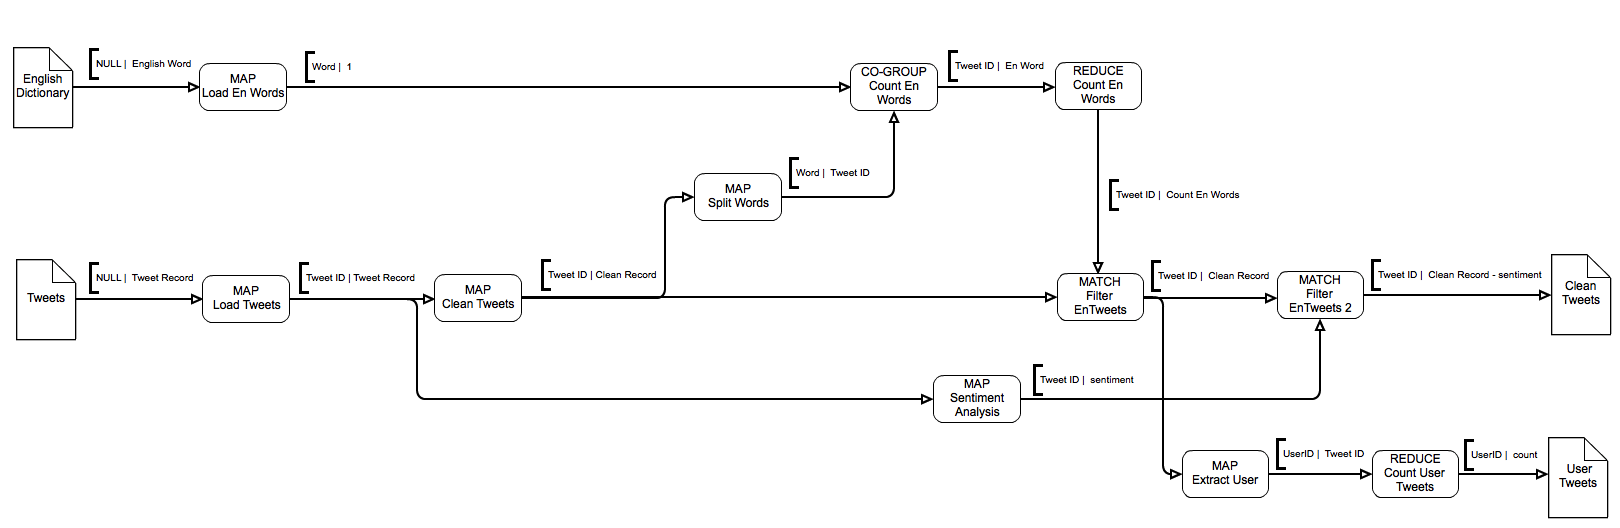
\includegraphics[width=\textwidth]{images/strato_pact_pt1.png} 
\caption{Data cleaning PACT}
\label{fig:cleaning}
\end{figure*}



\subsection{Compute statistics}

\begin{figure*}[t]
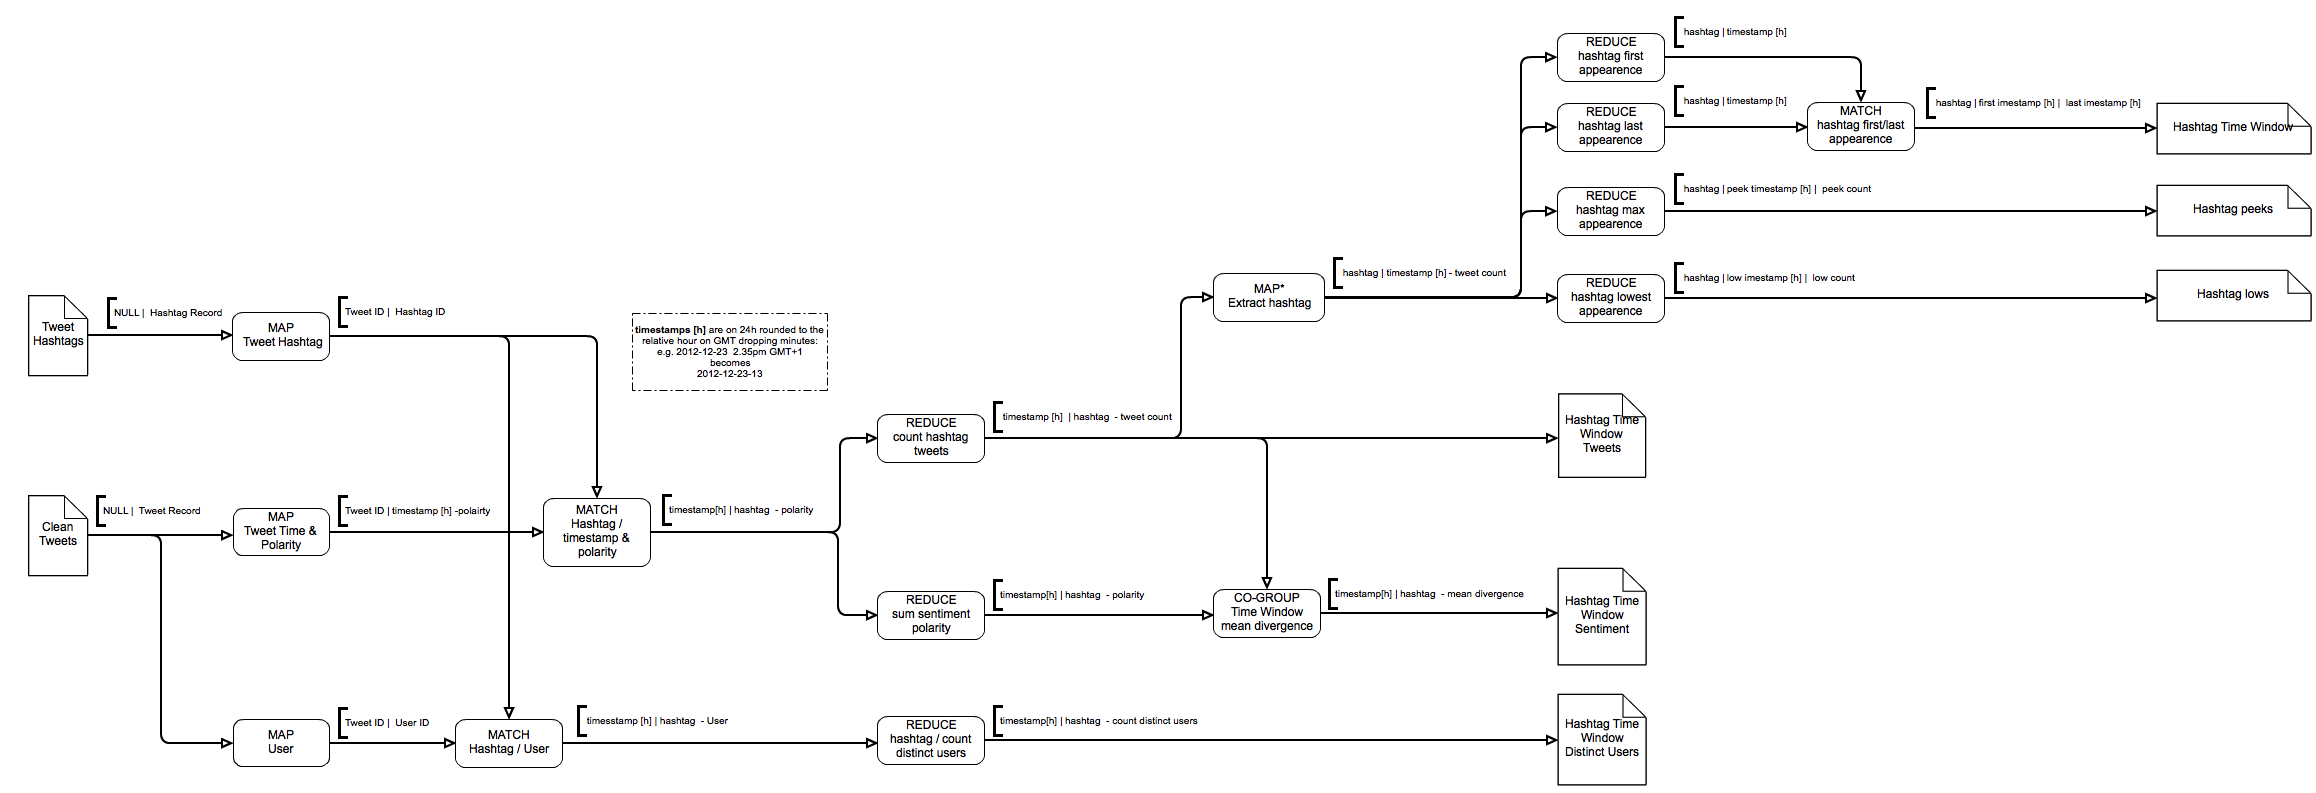
\includegraphics[width=\textwidth]{images/strato_pact_pt2.png} 
\caption{Compute statistics PACT}
\label{fig:statistics}
\end{figure*}

\section{Experimental evaluation}
\section{Conclusions}

%\nocite{Garey:1990:CIG:574848}
%\nocite{amer2004}

%\appendix
%\input{thoughts}
%\input{problem}
%\balancecolumns

%\clearpage

\def\thebibliography#1{
  \section*{References}
 %\normalsize                  % smaller; put \normalsize after bib --dt
 %\small
 \scriptsize
  \list
    {[\arabic{enumi}]}
    {\settowidth\labelwidth{[#1]}
     \leftmargin\labelwidth
     \parsep 1pt                % tighter --dt
     \itemsep 0.6pt               % tighter --dt
     \advance\leftmargin\labelsep
     \usecounter{enumi}
    }
  \def\newblock{\hskip .11em plus .33em minus .07em}
  \sloppy\clubpenalty10000\widowpenalty10000
  \sfcode`\.=1000\relax
}
\bibliographystyle{abbrv}
\bibliography{paperbib}  


\end{document}
